\documentclass[11pt, spanish]{article}
\usepackage[spanish]{babel}
\selectlanguage{spanish}
\usepackage{natbib}
\usepackage{url}
\usepackage[utf8x]{inputenc}
\usepackage{graphicx}
\graphicspath{{images/}}
\usepackage{parskip}
\usepackage{fancyhdr}
\usepackage{vmargin}
\usepackage{multirow}
\usepackage{float}
\usepackage{chngpage}

\usepackage{subcaption}

\usepackage{hyperref}
\usepackage[
    type={CC},
    modifier={by-nc-sa},
    version={4.0},
]{doclicense}

\hypersetup{
    colorlinks=true,
    linkcolor=blue,
    filecolor=magenta,      
    urlcolor=cyan,
}

% para codigo
\usepackage{listings}
\usepackage{xcolor}



%% configuración de listings

\definecolor{listing-background}{HTML}{F7F7F7}
\definecolor{listing-rule}{HTML}{B3B2B3}
\definecolor{listing-numbers}{HTML}{B3B2B3}
\definecolor{listing-text-color}{HTML}{000000}
\definecolor{listing-keyword}{HTML}{435489}
\definecolor{listing-identifier}{HTML}{435489}
\definecolor{listing-string}{HTML}{00999A}
\definecolor{listing-comment}{HTML}{8E8E8E}
\definecolor{listing-javadoc-comment}{HTML}{006CA9}

\lstdefinestyle{eisvogel_listing_style}{
  language         = lisp,
%$if(listings-disable-line-numbers)$
%  xleftmargin      = 0.6em,
%  framexleftmargin = 0.4em,
%$else$
  numbers          = left,
  xleftmargin      = 0em,
 framexleftmargin = 0em,
%$endif$
  backgroundcolor  = \color{listing-background},
  basicstyle       = \color{listing-text-color}\small\ttfamily{}\linespread{1.15}, % print whole listing small
  breaklines       = true,
  frame            = single,
  framesep         = 0.19em,
  rulecolor        = \color{listing-rule},
  frameround       = ffff,
  tabsize          = 4,
  numberstyle      = \color{listing-numbers},
  aboveskip        = 1.0em,
  belowskip        = 0.1em,
  abovecaptionskip = 0em,
  belowcaptionskip = 1.0em,
  keywordstyle     = \color{listing-keyword}\bfseries,
  classoffset      = 0,
  sensitive        = true,
  identifierstyle  = \color{listing-identifier},
  commentstyle     = \color{listing-comment},
  morecomment      = [s][\color{listing-javadoc-comment}]{/**}{*/},
  stringstyle      = \color{listing-string},
  showstringspaces = false,
  escapeinside     = {/*@}{@*/}, % Allow LaTeX inside these special comments
  literate         =
  {á}{{\'a}}1 {é}{{\'e}}1 {í}{{\'i}}1 {ó}{{\'o}}1 {ú}{{\'u}}1
  {Á}{{\'A}}1 {É}{{\'E}}1 {Í}{{\'I}}1 {Ó}{{\'O}}1 {Ú}{{\'U}}1
  {à}{{\`a}}1 {è}{{\'e}}1 {ì}{{\`i}}1 {ò}{{\`o}}1 {ù}{{\`u}}1
  {À}{{\`A}}1 {È}{{\'E}}1 {Ì}{{\`I}}1 {Ò}{{\`O}}1 {Ù}{{\`U}}1
  {ä}{{\"a}}1 {ë}{{\"e}}1 {ï}{{\"i}}1 {ö}{{\"o}}1 {ü}{{\"u}}1
  {Ä}{{\"A}}1 {Ë}{{\"E}}1 {Ï}{{\"I}}1 {Ö}{{\"O}}1 {Ü}{{\"U}}1
  {â}{{\^a}}1 {ê}{{\^e}}1 {î}{{\^i}}1 {ô}{{\^o}}1 {û}{{\^u}}1
  {Â}{{\^A}}1 {Ê}{{\^E}}1 {Î}{{\^I}}1 {Ô}{{\^O}}1 {Û}{{\^U}}1
  {œ}{{\oe}}1 {Œ}{{\OE}}1 {æ}{{\ae}}1 {Æ}{{\AE}}1 {ß}{{\ss}}1
  {ç}{{\c c}}1 {Ç}{{\c C}}1 {ø}{{\o}}1 {å}{{\r a}}1 {Å}{{\r A}}1
  {€}{{\EUR}}1 {£}{{\pounds}}1 {«}{{\guillemotleft}}1
  {»}{{\guillemotright}}1 {ñ}{{\~n}}1 {Ñ}{{\~N}}1 {¿}{{?`}}1
  {…}{{\ldots}}1 {≥}{{>=}}1 {≤}{{<=}}1 {„}{{\glqq}}1 {“}{{\grqq}}1
  {”}{{''}}1
}
\lstset{style=eisvogel_listing_style}


\usepackage[default]{sourcesanspro}

\setmarginsrb{2 cm}{1 cm}{2 cm}{2 cm}{1 cm}{1.5 cm}{1 cm}{1.5 cm}

\title{Práctica 3:\\
 Representación de dominios y resolución de\\ problemas con técnicas de planificación  \hspace{0.05cm} }                           
\author{Antonio David Villegas Yeguas}                             
\date{\today}                                           


\makeatletter
\let\thetitle\@title
\let\theauthor\@author
\let\thedate\@date
\makeatother

\pagestyle{fancy}
\fancyhf{}
\rhead{\theauthor}
\lhead{\thetitle}
\cfoot{\thepage}

\begin{document}

%%%%%%%%%%%%%%%%%%%%%%%%%%%%%%%%%%%%%%%%%%%%%%%%%%%%%%%%%%%%%%%%%%%%%%%%%%%%%%%%%%%%%%%%%

\begin{titlepage}
    \centering
    \vspace*{0.3 cm}
    
\includegraphics[scale = 0.50]{ugr.png}\\[0.7 cm]
    %\textsc{\LARGE Universidad de Granada}\\[2.0 cm]   
    \textsc{\large 3º CSI 2019/20 - Grupo 1}\\[0.5 cm]            
    \textsc{\large Grado en Ingeniería Informática}\\[0.5 cm]              
    \rule{\linewidth}{0.2 mm} \\[0.2 cm]
    { \huge \bfseries \thetitle}\\
    \rule{\linewidth}{0.2 mm} \\[1 cm]
    
    \begin{minipage}{0.4\textwidth}
        \begin{flushleft} \large
            \emph{Autor:}\\
            \theauthor\\ 
			 \emph{DNI:}\\
            77021623-M
            \end{flushleft}
            \end{minipage}~
            \begin{minipage}{0.4\textwidth}
            \begin{flushright} \large
            \emph{Asignatura: \\
            Técnicas de los Sistemas Inteligentes}   \\     
            \emph{Correo:}\\
            advy99@correo.ugr.es           
        \end{flushright}
    \end{minipage}\\[0.5cm]
  
    {\large \thedate}\\[0.5cm]
    %{\url{https://github.com/advy99/TSI/}}
    {\doclicenseThis}
 	
    \vfill
    
\end{titlepage}

%%%%%%%%%%%%%%%%%%%%%%%%%%%%%%%%%%%%%%%%%%%%%%%%%%%%%%%%%%%%%%%%%%%%%%%%%%%%%%%%%%%%%%%%%

%\tableofcontents
%\pagebreak

%%%%%%%%%%%%%%%%%%%%%%%%%%%%%%%%%%%%%%%%%%%%%%%%%%%%%%%%%%%%%%%%%%%%%%%%%%%%%%%%%%%%%%%%%

\section*{Introducción}

El objetivo de esta práctica consiste en diseñar e implementar un dominio de planificación clásico basado en el videojuego StarCraft. Para cada ejercicio tendremos que implementar dos ficheros en el lenguaje PDDL, uno para describir el dominio del ejercicio y otro para definir el problema. Para ejecutar los ejercicios utilizaremos el planificador Metric-FF para obtener el plan.

En el dominio declararemos todos los requisitos, tipos, constantes, funciones, predicados y acciones que se podrá tener o realizar nuestro mundo, mientras que en el problema declararemos objetos, especificaremos su estado inicial en el mundo basándonos en el dominio y estableceremos una meta. El objetivo de cada ejercicio es obtener un plan para que en el mundo basado en el dominio se cumpla dicha meta.

Cada ejercicio está basado en el anterior, por lo que los ficheros estarán basados e incluirán todo lo del ejercicio anterior a no ser que se especifique que se ha modificado.  Aun así, para distinguir el dominio y problema de cada ejercicio usare como nombre de dominio ejercicio\_N y como nombre del problema ejercicioN, por ejemplo, para el ejercicio 1 el dominio se llamará ejercicio\_1 y el problema será problema1.

\section{Ejercicio 1}

Para este ejercicio implementaré toda la base que utilizaremos para el resto de los ejercicios, por lo que el resto de ejercicios serán modificaciones del ejercicio anterior. 

En este ejercicio se nos pide representar los tipos básicos, constantes para referirnos a algunos de esos tipos, distintos predicados y tres acciones distintas, todo esto lo comentaré más en detalle en el desarrollo de su implementación. Una vez que tengamos dicho dominio definido se nos pide crear un problema de un mapa 5x5 donde se encuentre un centro de mando, tres unidades VCE, tres nodos de Mineral y dos de Gas. Se nos pide como objetivo construir un edificio Barracones.


\subsection{Dominio}

Para empezar, al definir el fichero de dominio declararemos los requisitos del dominio usando la sección \texttt{:requirements}, que serán los que se nos pide en todos los ejercicios, es decir, strips, adl y fluents.

\subsubsection{Tipos:}

Tras esto definimos los tipos que se nos pide para desarrollar la práctica. Usaremos los siguientes tipos que definiremos en la sección \texttt{:types}:

\begin{enumerate}
	\item localizacion: subtipo de object
	\item entidad: subtipo de object
	\item recurso: subtipo de object
	\item edificio: subtipo de entidad
	\item unidad: subtipo de entidad
	\item tipoRecurso: subtipo de recurso
	\item tipoEdificio: subtipo de edificio
	\item tipoUnidad: subtipo de unidad
\end{enumerate}

Los edificios y unidades, al poder estar posicionadas en distintas localizaciones y como, veremos en los siguientes ejercicios, tener predicados en común, serán ambos un subtipo de entidad, de forma que, por ejemplo, para saber si un edificio o una unidad está en una localización utilizaremos el tipo entidad para referirnos a cualquiera de estos dos tipos.

Al hacer uso de constantes para referirnos a las clases en las acciones y algunos predicados usaremos las clases que tienen prefijo tipo, esto lo haremos para enlazar las constantes con los objetos del problema y así poder generalizar en lugar de generar muchos objetos en el problema cuando podemos referirnos a estos como constantes.


\subsubsection{Constantes:}

Definidas en la sección \texttt{:constants}. Utilizaremos constantes para en el dominio poder referirnos a todos los objetos de un tipo, evitando tener que declarar los objetos en el problema y por tanto obtener una solución más generalizada para los problemas, las constantes que usaremos serán:

\begin{enumerate}
	\item VCE: de tipo tipoUnidad
	\item CentroDeMando: de tipo tipoEdificio
	\item Barracones: de tipo tipoEdificio
	\item Mineral: de tipo tipoRecurso
	\item Gas: de tipo tipoRecurso
\end{enumerate}


\subsubsection{Predicados:}


Definidas en la sección \texttt{:predicates}. Los predicados serán los que definan el estado del mundo, el entorno. Para definir el mundo podemos utilizar estos predicados:

\begin{itemize}
	\item (entidadEnLocalizacion ?obj - entidad x - localizacion): Nos servirá para representar que una en localización se encuentra una entidad, ya sea un edificio o una unidad.
	\item (caminoEntre ?x - localizacion ?y - localizacion): Nos servirá para representar que dos localizaciones están conectadas.
	\item (asignarNodoRecursoLocalizacion ?r - recurso ?x - localizacion): Servirá para representar que en una localización hay un nodo de recurso.
	\item (estaExtrayendoRecurso ?rec - recurso): Para representar que se extra extrayendo un recurso.
	\item (necesitaRecurso ?x - tipoEdificio ?rec - tipoRecurso): Para representar que cierto edificio necesita cierto recurso para ser construido.
	\item (unidadLibre ?u - unidad): Para representar que cierta unidad del problema está libre (no está asignada a un recurso).
	\item (esEdificio ?edif - edificio ?tEdif - tipoEdificio): Representa que un edificio es de un tipo.
	\item (esUnidad ?u - unidad ?tU - tipoUnidad): Representa que una unidad es de un tipo.
	
\end{itemize}

Con estos predicados representaremos el mundo, y además, en conjunto con otros predicados, podremos inferir otras cosas, como por ejemplo, si una unidad no está libre y está en el mismo lugar que un nodo de Gas, esa unidad está extrayendo Gas, de ahí que no tengamos el predicado para saber si cierta unidad está extrayendo en cierta posición.

\subsubsection{Acciones:}

Cada una definida en una sección \texttt{:action}. En este primer ejercicio se pueden realizar tres acciones: navegar por el mapa, asignar un VCE a extraer un recurso y construir un edificio. Cada acción para poder ser realizada necesitará cumplir ciertas precondiciones, y cada acción tendrá ciertos efectos.

\begin{itemize}
	\item Navegar: Recibe como parámetros una unidad (?u) y dos localizaciones (?x ?y). Como precondiciones la unidad tiene que estar en la primera localización (entidadEnLocalizacion ?u ?x), tiene que existir un camino entre las dos localizaciones (caminoEntre ?x ?y) y la unidad tiene que estar libre (unidadLibre ?u). Como efecto, la unidad deja de estar en la primera localización (not (entidadEnLocalizacion ?u ?x)) y pasa a estar en la segunda (entidadEnLocalizacion ?u ?y).
	\item Asignar: Recibe como parámetros una unidad (?u), un recurso (?r) y una localización (?x). Como precondiciones, la unidad tiene que estar en la localización dada (entidadEnLocalizacion ?u ?x), la localización tiene que tener un nodo del recurso dado (asignarNodoRecursoLocalizacion ?r ?l) y la unidad tiene que estar libre (unidadLibre ?u). Como efecto la unidad deja de esta libre (not (unidadLibre ?u)) y se está extrayendo el recurso (estaExtrayendoRecurso ?rec).
	\item Construir: Recibe como parámetros una unidad (?u), una localización (?x), un edificio (?e) y un recurso (?r). Como precondición la unidad ha de estar libre (unidadLibre ?u), la unidad tiene que estar en dicha localización (entidadEnLocalización ?u ?x) y además existe un tipo de edificio (?tEdif), el edificio dado es del tipo ?t (esEdificio ?e ?t) tal que ese tipo de edificio necesita el recurso dado (necesitaRecurso ?t ?r) y además se está extrayendo (estaExtrayendo ?r). Como efecto, la entidad del edificio está en la localización dada. (entidadEnLocalizacion ?e ?x)
\end{itemize}


Con todos estos tipos, constantes y posibles acciones podemos definir un problema con el que, usando las acciones, Metric-FF encuentre una secuencia de acciones que resuelvan el problema.

\subsection{Problema}

El fichero del problema se compone de cinco partes esenciales:

\subsubsection{Dominio:}

Se representa usando \texttt{(:domain dominio)} en PDDL. Esta sección indica el dominio donde estará definido el problema, en nuestro caso será el dominio ejercicio\_1.

\subsubsection{Objetos:}

Se representa usando \texttt{:objects} en PDDL. En esta sección declararemos todos los objetos que intervienen en el problema.

Para empezar declararemos 25 objetos de tipo localización para representar el mapa.

También declararemos tres VCE de tipo unidad, un centro de mando de tipo edificio y unos barracones de tipo edificio, y con esto hemos declarado todos los objetos que nos pide el problema.

Es importante que aunque como veremos más adelante, los barracones es el objetivo a construir, sin embargo han de ser declarados como objeto para que sea capaz de construir dicho objeto.


\subsubsection{Estado inicial:}

Se representa usando \texttt{:init} en PDDL. En esta sección declararemos el estado inicial de los objetos usando los predicados del dominio.

Para empezar representaremos todas las conexiones entre localizaciones. Para esto hemos usado el editor online de PDDL haciendo uso de la extensión propuesta en los foros de dudas para la práctica en PRADO.

Además hemos establecido posiciones iniciales arbitrarias para las tres unidades VCE y el centro de mando, así como establecido los nodos de recursos. Las posiciones de los recursos las hemos establecido haciendo uso de las constantes, de forma que no es necesario declarar tres minerales y dos objetos de tipo gas. También he establecido el tipo de las unidades y los edificios usados para enlazarlos con sus constantes, así como los recursos que necesita cada edificio según nos marca el guión.

Todo esto se realiza con los predicados del dominio, explicados en los apartados anteriores.

\subsubsection{Meta:}

Se representa usando \texttt{:goal} en PDDL. Esta sección servirá para definir el objetivo del plan, es decir, PDDL intentará encontrar un plan (sucesión de acciones) que haga verdadero la meta. Para este ejercicio es que el objeto barracones esté en una posición escogida de forma arbitraria.

\subsubsection{Métrica:}

Se representa usando \texttt{:metric} en PDDL. En principio no utilizaremos esta sección hasta el último ejercicio. Usando esta sección podemos establecer una métrica propia. Por defecto la métrica es minimizar la longitud del plan, es decir, obtener el plan que necesite menos acciones.


\subsection{Solución:}

Tras declarar el dominio y el problema, al ejecutar los ficheros PDDL sobre Metric-FF obtenemos el siguiente plan:

\begin{figure}[H]
	\centering
	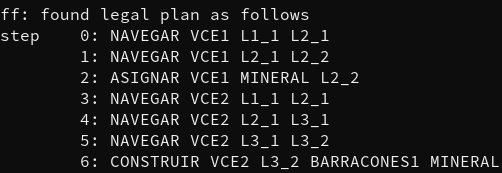
\includegraphics[scale=0.4]{plan1.png}
	\caption{Plan obtenido en el ejercicio 1.}
	\label{plan1}
\end{figure}

\section{Ejercicio 2}

Para este ejercicio se nos pide modificar el anterior para que solo se pueda extraer el recurso Gas si se dispone de un nuevo edificio, el Extractor, en un nodo de Gas.

Al ser una modificación del ejercicio anterior solo indicaré los cambios.

\subsection{Dominio:}

\subsubsection{Constantes:}

Se ha añadido una nueva constante para representar el nuevo edificio: Extractor, de tipo tipoEdificio.

\subsubsection{Acciones:}

Se ha modificado la acción Asignar. Ahora recibe un nuevo parámetro ?edi - edificio. Este parámetro lo usaremos para comprobar que si se va a extraer Gas, en la localización existe el edificio dado por parámetro y es un edificio Extractor.

Para comprobar esta nueva precondición usaremos la orden imply, equivalente al operador lógico de la implicación:

\begin{lstlisting}
(imply (a) (b) )
\end{lstlisting}

Utilizar este operador es equivalente a realizar la comprobación $\neg a \lor b$. En nuestro caso $a$ será  (asignarNodoRecursoLocalzizacion Gas ?x), de forma que si en la localización no hay un nodo de Gas no tiene porque cumplirse $b$, sin embargo, si es Gas se tiene que cumplir $b$, que será (and (entidadEnLocalizacion ?edi ?x) (esEdificio ?edi Extractor) para comprobar que tenemos el edificio dado en la localización, y ese edificio es de tipo Extractor.

\subsection{Problema:}

\subsubsection{Objetos:}

Ahora será necesario declarar al menos un objeto extractor por si necesita construirse en algún momento.

\subsubsection{Estado inicial:}

El estado inicial será el mismo, solo que añadiendo la inicialización para representar que el extractor.

\subsubsection{Meta:}

El objetivo de este ejercicio es el mismo que el del ejercicio anterior. Debido a que para construir los barracones no es necesario Gas y no se puede comprobar que construye el extractor de forma correcta, he realizado pruebas usando de meta que el objetivo sea estar extrayendo Gas para comprobar que funciona.

\subsection{Solución:}

Tras ejecutarlo con Metric-FF obtenemos:


\begin{figure}[H]
	\centering
	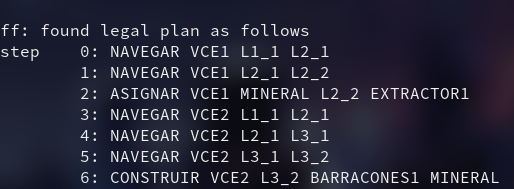
\includegraphics[scale=0.4]{plan2.png}
	\caption{Plan obtenido en el ejercicio 2.}
	\label{plan1}
\end{figure}

Y como vemos, al no extraer Gas, no construye el extractor, para comprobar que funciona he realizado una modificación en la meta (la versión entregada tiene la meta pedida en el guión, no esta modificación):


\begin{figure}[H]
	\centering
	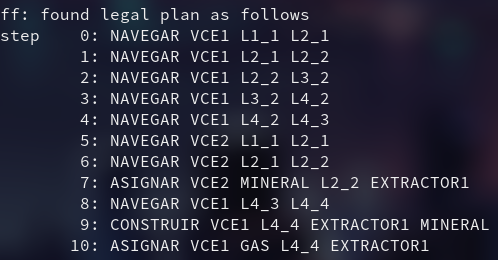
\includegraphics[scale=0.4]{plan2Gas.png}
	\caption{Plan obtenido en el ejercicio 2 con la meta modificada.}
	\label{plan1}
\end{figure}

Y podemos ver como antes de extraer Gas es construido el Extractor.

\section{Ejercicio 3}

En este ejercicio tenemos que modificar la acción Construir para tener en cuenta que un edificio puede necesitar varios recursos.

\section{Ejercicio 4}


\section{Ejercicio 5}



\section{Ejercicio 6}


\section{Ejercicio 7}

\end{document}
